\documentclass[12pt]{article}
\usepackage[table]{xcolor}
\usepackage[shortlabels]{enumitem}
\usepackage{tabularx,xltabular}
\usepackage{graphicx}
\usepackage{hyperref}
\usepackage{verbatim}
\usepackage{geometry}
\usepackage{ulem}
\usepackage[official]{eurosym}
\usepackage{tikz}
\usetikzlibrary{arrows,backgrounds,calc,decorations.markings,patterns,3d,positioning,fit,angles, quotes}
\usepackage{pgfplots}
\pgfplotsset{compat = newest}
\usetikzlibrary{fit}
\newcommand\addvmargin[1]{
\usetikzlibrary{arrows}
\node[fit=(current bounding box),inner ysep=#1,inner xsep=0]{};}
\usepackage{cancel}
\usepackage{fontspec}
\usepackage{array}  
\geometry{a4paper, top=2cm, left=2cm, right=2cm, bottom=2cm, headsep=1cm}
\usepackage{tabu}
\usepackage{pst-node}
\usepackage{colortbl}
\usepackage{array}
\usepackage{german}
\setlength\parindent{0pt}
\newcolumntype{?}{!{\vrule width 1pt}}
\usepackage{makecell}
\renewcommand{\arraystretch}{2.5}
\usepackage{pbox}
\usepackage{amssymb}
\usepackage{amsmath}
\usepackage{booktabs}
\newcolumntype{L}[1]{>{\raggedright\let\newline\\\arraybackslash\hspace{0pt}}m{#1}}
\newcolumntype{C}[1]{>{\centering\let\newline\\\arraybackslash\hspace{0pt}}m{#1}}
\newcolumntype{R}[1]{>{\raggedleft\let\newline\\\arraybackslash\hspace{0pt}}m{#1}}
\begin{document}
\rightline{Datum: 08.12.2023}
\centerline{{\Large Üben für die Arbeit}} 
\vspace{1cm}
\noindent \\


\begin{xltabular}{\textwidth}{|C{0.75cm}|X|}
\arrayrulecolor{black}\hline
a)&Setze für die Variabel a den Wert 3 ein und berechne den Wert des Terms:$$4 - 2 \cdot a$$
\\\hline
b)&Setze für die Variabel b den Wert 4 ein und berechne den Wert des Terms:$$2 \cdot b + 3 \cdot b$$
\\\hline
c)&Vereinfache:$$4 - 4b - 4b=?$$
\\\hline
d)&Vereinfache:$$2 + 2=?$$
\\\hline
e)&Berechne die Variable $$5\cdot y-7=43$$
\\\hline
f)&Berechne die Variable $$3\cdot a-15=0$$
\\\hline
g)&\pbox{6cm}{Bestimme den Umfang und die Fläche von: \\\tikzstyle{background grid}=[draw, black!15,step=.5cm]
\noindent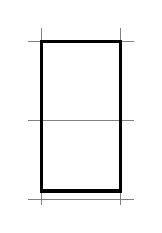
\begin{tikzpicture}[show background grid]
\draw[black, very thick] (0cm,0.1cm) rectangle (1cm,2cm);
\end{tikzpicture}}
\\\hline
h)&\pbox{5cm}{
Berechne den Flächeninhalt von:\\
\tikzstyle{background grid}=[draw, black!15,step=.5cm]
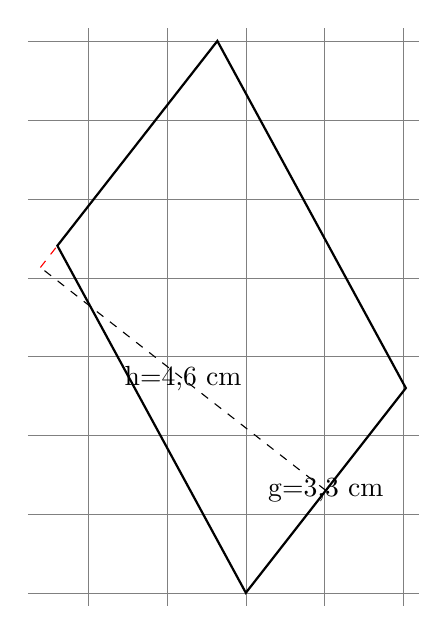
\begin{tikzpicture}[show background grid]
\draw[thick,black,rotate=52] (0,0) -- node{g=3,3 cm} ++(3.3,0) -- ++(2.0,4.6) -- ++(-3.3,0) --cycle;
\draw[dashed,black,rotate=52] (1.65,0)  -- node{h=4,6 cm} ++(0,4.6);
\draw[dashed,black,rotate=52,red] (1.65,4.6)  -- ++(0.3500000000000001,0);
\end{tikzpicture}
}
\\\hline
i)&\pbox{5cm}{
Berechne den Flächeninhalt von:\\
\tikzstyle{background grid}=[draw, black!15,step=.5cm]
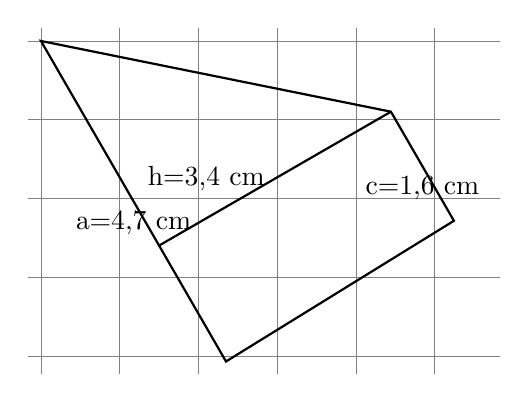
\begin{tikzpicture}[show background grid]
\draw[thick,black,rotate=300] (0,0) -- node[below]{a=4,7 cm} ++(4.7,0) -- ++(-0.1,3.4) --node[below]{c=1,6 cm} ++(-1.6,0) --cycle;
\draw[thick,black,rotate=300] (3.0,0) --node[left]{h=3,4 cm}  ++(0,3.4);
\end{tikzpicture}
}
\\\hline
j)&\pbox{5cm}{
Berechne den Flächeninhalt von:\\
\tikzstyle{background grid}=[draw, black!15,step=.5cm]
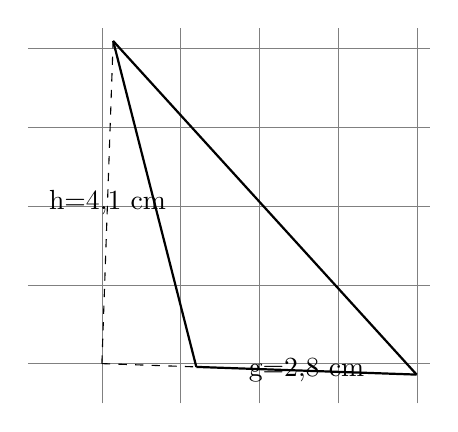
\begin{tikzpicture}[show background grid]
\draw[thick,black] (358:1.2000000000000002) -- node{g=2,8 cm} (358:4.0);
\draw[thick,black] (358:1.2000000000000002)  -- (448:4.1);
\draw[thick,black] (358:4.0)  -- (448:4.1);
\draw[dashed,black] (0,0)  -- node{h=4,1 cm} (448:4.1);
\draw[dashed,black] (0,0)  -- (358:1.2000000000000002);
\end{tikzpicture}
}
\\\hline
k)&\pbox{5cm}{
Berechne den Flächeninhalt von:\\
\tikzstyle{background grid}=[draw, black!15,step=.5cm]
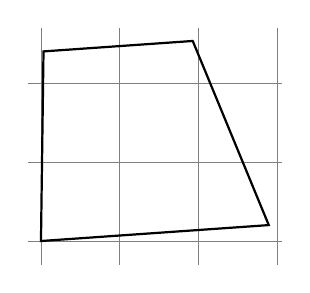
\begin{tikzpicture}[show background grid]
\draw[thick,black,rotate=4] (0,0) -- node[below]{} ++(2.9,0) -- ++(-0.8,2.4) --node[below]{} ++(-1.9,0) --cycle;
\end{tikzpicture}
}
\\\hline
l)&\pbox{5cm}{
Berechne den Flächeninhalt von:\\
\tikzstyle{background grid}=[draw, black!15,step=.5cm]
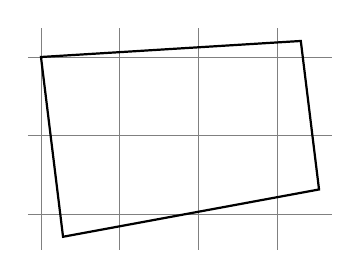
\begin{tikzpicture}[show background grid]
\draw[thick,black,rotate=277] (0,0) -- node[below]{} ++(2.3,0) -- ++(-0.2,3.3) --node[below]{} ++(-1.9,0) --cycle;
\end{tikzpicture}
}
\\\hline
m)&Stelle die Flächenformel des Parallelogramm nach der fehlenden Seite um und berechne diese und den Umfang für $A=13,77~cm^2$, $b=4,8~cm$ und $h_a=2,7~cm$.
\\\hline
n)&Stelle die Flächenformel des Rechtecks nach der fehlenden Seite um und berechne diese und den Umfang für $A=25,53~cm^2$ und $a=3,7~cm$.
\\\hline
\end{xltabular}
\vspace{0.5cm}
\newpage
\rightline{Datum: 08.12.2023}
\centerline{{\large Lösungen Üben für die Arbeit}} 
\vspace{0.5cm}

\begin{xltabular}{\textwidth}{|C{0.75cm}|X|C{0.75cm}|X|}
\arrayrulecolor{black}\hline
a)&$\begin{aligned}
\textcolor{red}{a=3} & \rightarrow\\
4 - 2 \cdot a=&4 - 2 \cdot \textcolor{red}{3}=-2\\
\end{aligned}$
&
b)&$\begin{aligned}
\textcolor{red}{b=4} & \rightarrow\\
2 \cdot b + 3 \cdot b=&2 \cdot \textcolor{red}{4} + 3 \cdot \textcolor{red}{4}=20\\
\end{aligned}$
\\\hline
c)&$4 - 4b - 4b=4 - 8b$
&
d)&$2 + 2=4$
\\\hline
e)&\begingroup\setlength{\jot}{-0.03cm}
\tikzstyle{background grid}=[draw, black!15,step=.5cm]
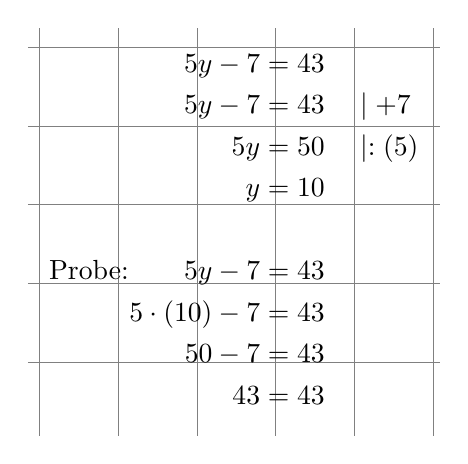
\begin{tikzpicture}[show background grid]
\node[below right] at (0,0.1) {
$\begin{aligned}
5y-7 &=43& &  \\
5y - 7 &=43& & \mid + 7\\
5y &=50& & \mid :\left(5\right)\\
y &=10& & 
\\
\\
\mbox{Probe:}\qquad 5y-7 &=43& &  \\
5\cdot \left(10\right)-7 &=43& &  \\
50-7 &=43& &  \\
43 &=43& &  \\
\end{aligned}$};
\end{tikzpicture}
\endgroup
&
f)&\begingroup\setlength{\jot}{-0.03cm}
\tikzstyle{background grid}=[draw, black!15,step=.5cm]
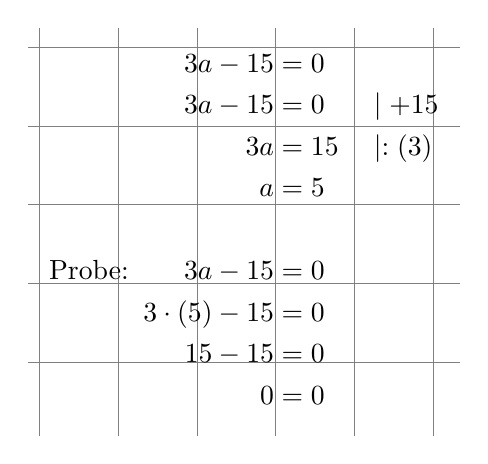
\begin{tikzpicture}[show background grid]
\node[below right] at (0,0.1) {
$\begin{aligned}
3a-15 &=0& &  \\
3a - 15 &=0& & \mid + 15\\
3a &=15& & \mid :\left(3\right)\\
a &=5& & 
\\
\\
\mbox{Probe:}\qquad 3a-15 &=0& &  \\
3\cdot \left(5\right)-15 &=0& &  \\
15-15 &=0& &  \\
0 &=0& &  \\
\end{aligned}$};
\end{tikzpicture}
\endgroup
\\\hline
g)&\pbox{6cm}{$U=2\cdot a+2\cdot b$ \\ $U=2\cdot1cm+2\cdot2cm=6cm$ \\$A=a\cdot b$ \\ $A=1\cdot2=2cm^2$ \\\tikzstyle{background grid}=[draw, black!15,step=.5cm]
\noindent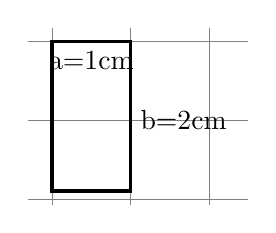
\begin{tikzpicture}[show background grid]
\draw[black, very thick] (0cm,0.1cm) rectangle (1cm,2cm);
\draw (0.5cm,2cm) node[below]{a=1cm}; 
\draw (1cm,1.0cm) node[right]{b=2cm}; 
\end{tikzpicture}}
&
h)&\pbox{5cm}{
$\begin{aligned}
geg.: g&=3,3 cm \\
   h&=4,6 cm \\
ges.: A&=? \\
A&=g\cdot h \\
&=3,3\cdot 4,6 \\
\makebox[0pt][l]{\uuline{\phantom{$A=15,18~cm^2$} } }
A&=15,18~cm^2
\end{aligned}$
\tikzstyle{background grid}=[draw, black!15,step=.5cm]
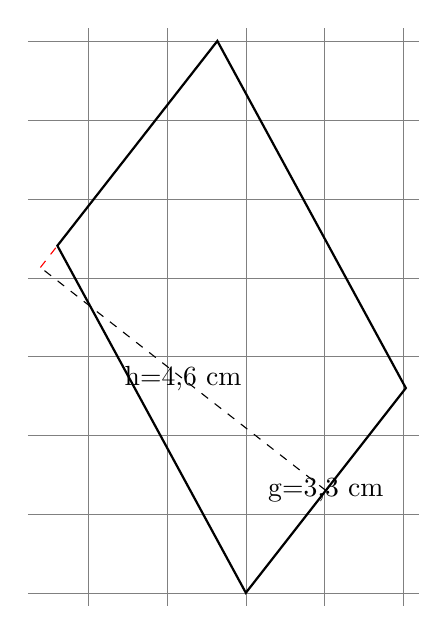
\begin{tikzpicture}[show background grid]
\draw[thick,black,rotate=52] (0,0) -- node{g=3,3 cm} ++(3.3,0) -- ++(2.0,4.6) -- ++(-3.3,0) --cycle;
\draw[dashed,black,rotate=52] (1.65,0)  -- node{h=4,6 cm} ++(0,4.6);
\draw[dashed,black,rotate=52,red] (1.65,4.6)  -- ++(0.3500000000000001,0);
\end{tikzpicture}
}
\\\hline
i)&\pbox{5cm}{
\tikzstyle{background grid}=[draw, black!15,step=.5cm]
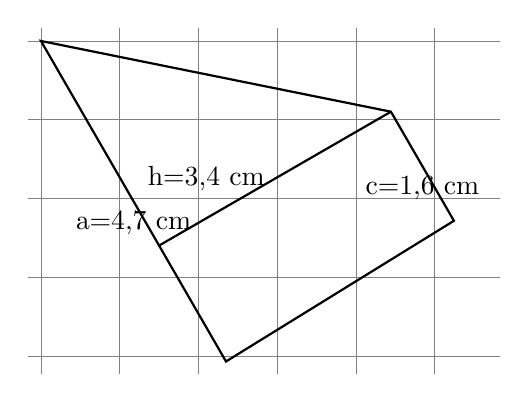
\begin{tikzpicture}[show background grid]
\draw[thick,black,rotate=300] (0,0) -- node[below]{a=4,7 cm} ++(4.7,0) -- ++(-0.1,3.4) --node[below]{c=1,6 cm} ++(-1.6,0) --cycle;
\draw[thick,black,rotate=300] (3.0,0) --node[left]{h=3,4 cm}  ++(0,3.4);
\end{tikzpicture}
$\begin{aligned}
geg.: a&=4,7 cm \\
   c&=1,6 cm \\
   h&=3,4 cm \\
ges.: A&=? \\
A&=\frac{a+c}{2}\cdot h \\
&=\frac{4,7+1,6}{2}\cdot3,4\\
\makebox[0pt][l]{\uuline{\phantom{$A=10,71~cm^2$} } }
A&=10,71~cm^2
\end{aligned}$
}
&
j)&\pbox{5cm}{
$\begin{aligned}
geg.: g&=2,8 cm \\
   h&=4,1 cm \\
ges.: A&=? \\
A&=\frac{g \cdot h}{2} \\
&=2,8 \cdot \frac{4,1}{2}\\
\makebox[0pt][l]{\uuline{\phantom{$A=5,74~cm^2$} } }
A&=5,74~cm^2
\end{aligned}$
\tikzstyle{background grid}=[draw, black!15,step=.5cm]
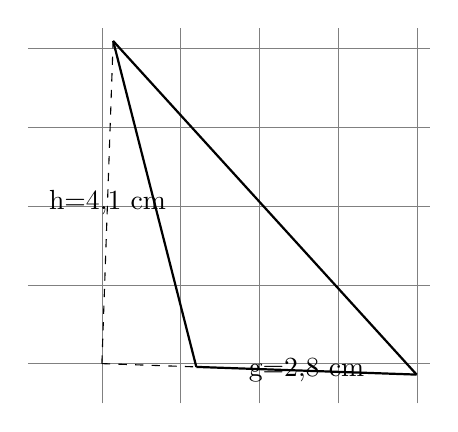
\begin{tikzpicture}[show background grid]
\draw[thick,black] (358:1.2000000000000002) -- node{g=2,8 cm} (358:4.0);
\draw[thick,black] (358:1.2000000000000002)  -- (448:4.1);
\draw[thick,black] (358:4.0)  -- (448:4.1);
\draw[dashed,black] (0,0)  -- node{h=4,1 cm} (448:4.1);
\draw[dashed,black] (0,0)  -- (358:1.2000000000000002);
\end{tikzpicture}
}
\\\hline
k)&\pbox{5cm}{
\tikzstyle{background grid}=[draw, black!15,step=.5cm]
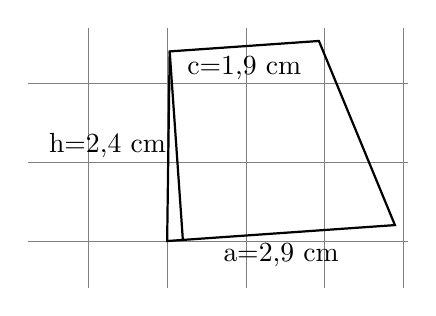
\begin{tikzpicture}[show background grid]
\draw[thick,black,rotate=4] (0,0) -- node[below]{a=2,9 cm} ++(2.9,0) -- ++(-0.8,2.4) --node[below]{c=1,9 cm} ++(-1.9,0) --cycle;
\draw[thick,black,rotate=4] (0.19999999999999996,0) --node[left]{h=2,4 cm}  ++(0,2.4);
\end{tikzpicture}
$\begin{aligned}
geg.: a&=2,9 cm \\
   c&=1,9 cm \\
   h&=2,4 cm \\
ges.: A&=? \\
A&=\frac{a+c}{2}\cdot h \\
&=\frac{2,9+1,9}{2}\cdot2,4\\
\makebox[0pt][l]{\uuline{\phantom{$A=5,76~cm^2$} } }
A&=5,76~cm^2
\end{aligned}$
}
&
l)&\pbox{5cm}{
\tikzstyle{background grid}=[draw, black!15,step=.5cm]
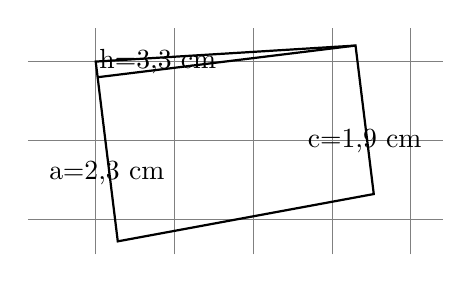
\begin{tikzpicture}[show background grid]
\draw[thick,black,rotate=277] (0,0) -- node[below]{a=2,3 cm} ++(2.3,0) -- ++(-0.2,3.3) --node[below]{c=1,9 cm} ++(-1.9,0) --cycle;
\draw[thick,black,rotate=277] (0.1999999999999999,0) --node[left]{h=3,3 cm}  ++(0,3.3);
\end{tikzpicture}
$\begin{aligned}
geg.: a&=2,3 cm \\
   c&=1,9 cm \\
   h&=3,3 cm \\
ges.: A&=? \\
A&=\frac{a+c}{2}\cdot h \\
&=\frac{2,3+1,9}{2}\cdot3,3\\
\makebox[0pt][l]{\uuline{\phantom{$A=6,93~cm^2$} } }
A&=6,93~cm^2
\end{aligned}$
}
\\\hline
m)&\tikzstyle{background grid}=[draw, black!15,step=.5cm]
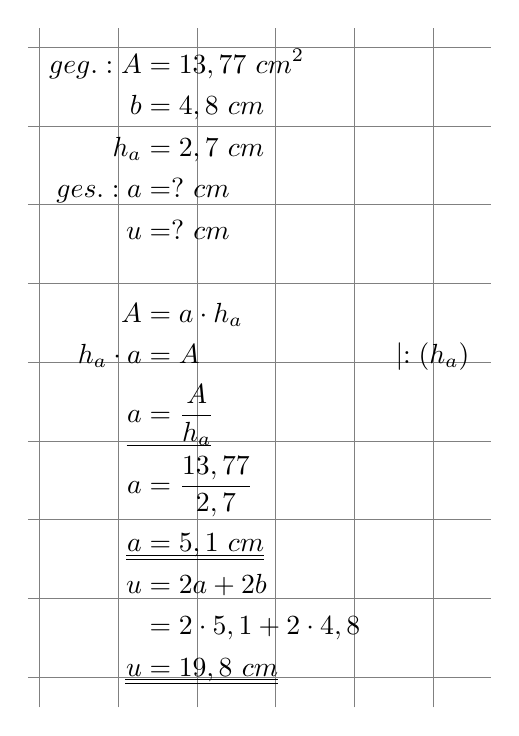
\begin{tikzpicture}[show background grid]
\node[below right] at (0,0.1) {
$\begin{aligned}
geg.: A &=13,77~cm^2& & \\
  b &=4,8~cm& & \\
  h_a &=2,7~cm& & \\
ges.: a &=?~cm& & \\
u &=?~cm& & \\
& & & \\
A &=a\cdot h_a& & \\
h_a\cdot a &=A& & \mid :(h_a)\\
\makebox(0pt,-0.25cm)[l]{\uline{\phantom{$a ={{\frac{A}{h_a}}}  \\$}}}
a &={{\frac{A}{h_a}}}& & \\
a&=\frac{13,77}{2,7}& & \\
\makebox[0pt][l]{\uuline{\phantom{$a=5,1~cm  \\$}}}
a&=5,1~cm& & \\
u&=2a+2b & & \\
&=2\cdot5,1+2\cdot4,8& & \\
\makebox[0pt][l]{\uuline{\phantom{$u=19,8~cm     \\$}}}
u&=19,8~cm   & & \\
\end{aligned}$};
\end{tikzpicture}
&
n)&\tikzstyle{background grid}=[draw, black!15,step=.5cm]
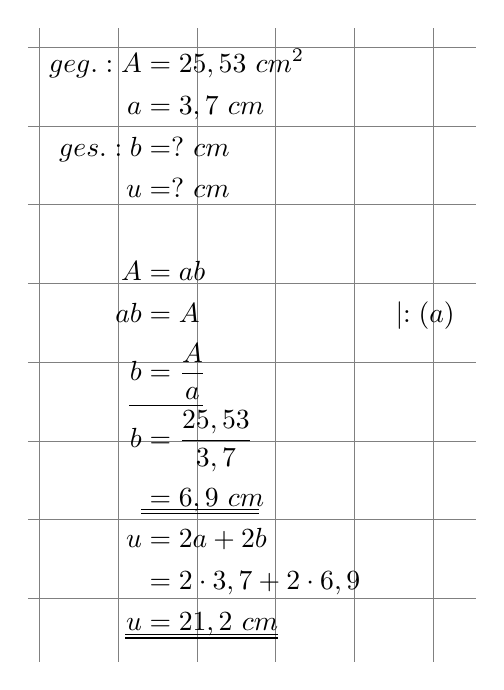
\begin{tikzpicture}[show background grid]
\node[below right] at (0,0.1) {
$\begin{aligned}
geg.: A &=25,53~cm^2& & \\
  a &=3,7~cm& & \\
ges.: b &=?~cm& & \\
u &=?~cm& & \\
& & & \\
A &=ab& & \\
ab &=A& & \mid :(a)\\
\makebox(0pt,-0.25cm)[l]{\uline{\phantom{$b ={{\frac{A}{a}}}  \\$}}}
b &={{\frac{A}{a}}}& & \\
b&=\frac{25,53}{3,7}& & \\
\makebox[0pt][l]{\uuline{\phantom{$=6,9~cm  \\$}}}
&=6,9~cm& & \\
u&=2a+2b & & \\
&=2\cdot3,7+2\cdot6,9& & \\
\makebox[0pt][l]{\uuline{\phantom{$u=21,2~cm     \\$}}}
u&=21,2~cm   & & \\
\end{aligned}$};
\end{tikzpicture}
\\\hline
\end{xltabular}
\vspace{0.5cm}
\end{document}